
\documentclass[10pt, conference, compsocconf]{IEEEtran}  
                                                         


\IEEEoverridecommandlockouts                             
                                                         
                                                         
\overrideIEEEmargins

\usepackage[latin1]{inputenc}
\usepackage{makecell}
\usepackage{graphicx}
\usepackage{blindtext, graphicx}
\usepackage{multirow}
%\usepackage{algorithm}
\usepackage{algpseudocode}
\algdef{SE}[DOWHILE]{Do}{doWhile}{\algorithmicdo}[1]{\algorithmicwhile\ #1}%
\setcounter{secnumdepth}{4}
\usepackage[linesnumbered,ruled,vlined]{algorithm2e} 
\usepackage[first=0,last=9]{lcg}
\usepackage{color, colortbl}
\definecolor{Gray}{gray}{0.9}
\usepackage{tabularx} % in the preamble
\usepackage{tabu}
\usepackage{booktabs}
\usepackage[tight,footnotesize]{subfigure}

\newcolumntype{P}[1]{>{\centering\arraybackslash}p{#1}}
\newcolumntype{M}[1]{>{\centering\arraybackslash}m{#1}}
\newcommand{\head}[1]{\textnormal{\textbf{#1}}}


\title{\LARGE \bf
Host Hypervisor Trace Mining for Virtual Machine Workload Characterization
}


\author{\IEEEauthorblockN{Hani Nemati\IEEEauthorrefmark{1}, Seyed Vahid Azhari\IEEEauthorrefmark{2}, and Michel R. Dagenais\IEEEauthorrefmark{3}}
\IEEEauthorblockA{Department of Computer and Software Engineering,\\ Polytechnique Montreal, Quebec, Canada \\
Email: \{\IEEEauthorrefmark{1}hani.nemati@polymtl.ca,\IEEEauthorrefmark{2}azharivs@gmail.com,\IEEEauthorrefmark{3}michel.dagenais@polymtl.ca}}


\begin{document}



\maketitle
\thispagestyle{empty}
\pagestyle{empty}


%%%%%%%%%%%%%%%%%%%%%%%%%%%%%%%%%%%%%%%%%%%%%%%%%%%%%%%%%%%%%%%%%%%%%%%%%%%%%%%%
\begin{abstract}

The efficient operation and resource management of multi-tenant data centers hosting thousands of services is a demanding task that requires precise and detailed information regarding the behaviour of each and every virtual machine (VM). Often, coarse measures such as CPU, memory, disk and network usage by VMs are considered in grouping them onto the same physical server, as detailed measures would require access to the guest operating system (OS) which is not feasible in a multi-tenant setting.

In this paper, we propose host level hypervisor tracing as a non-intrusive means to extract useful features that can provide for fine grain characterization of VM behaviour. In particular, we extract VM blocking periods as well as virtual interrupt injection rates to detect multiple levels of resource intensiveness. In addition, we consider resource contention rate due to other VMs and the host, along with reasons for exit from non-root to root privileged mode revealing useful information about the nature of the underlying VM workload. We also use tracing to get information about rate of process and thread preemption in each VM extracting process and thread contention as another feature set. We then employ various feature selection strategies and assess the quality of the resulting workload clustering. Notably, we adopt a two stage feature selection approach in addition to a one shot clustering scheme. Moreover, we consider inter-cluster and intra-cluster similarity metrics such as silhouette score to discover distinct groups of workloads as well as workload groups with significant overlap. This information can be used by 1) data center administrators to gain deep visibility into the nature of various VMs running on their infrastructure, 2) performance engineers to assist root cause analysis of VM issues and 3) IaaS provider to help in resource management based on VM behavior. 


\end{abstract}


\begin{IEEEkeywords}
VM Clustering, Workload characterization, performance analysis, tracing, vCPU states, K-Means, Machine Learning.
\end{IEEEkeywords}

%%%%%%%%%%%%%%%%%%%%%%%%%%%%%%%%%%%%%%%%%%%%%%%%%%%%%%%%%%%%%%%%%%%%%%%%%%%%%%%%
\section{Introduction}

Introduction goes here. 

%%%%%%%%%%%%%%%%%%%%%%%%%%%%%%%%%%%%%%%%%%%%%%%%%%%%%%%%%%%%%%%%%%%%%%%%%%%%%%%%
\section{Related Work}



%%%%%%%%%%%%%%%%%%%%%%%%%%%%%%%%%%%%%%%%%%%%%%%%%%%%%%%%%%%%%%%%%%%%%%%%%%%%%%%%


\section{VM Features and Types Selection}

\subsection{VM Machine States Analysis}

Intel processors (like AMD processors) provide support for virtualization by Virtual Machine eXtensions (VMX) instructions set (AMD
supports Secure Virtual Machine (SVM) instructions set). There are two types of VMX operation: \textbf{VMX root} operation and \textbf{VMX non-root} operation.  Privileged instruction executed by VM causes a VM exit to VMX root mode to pass the control to Virtual Machine Monitor (VMM) in order to execute the instruction in a safe environment.  After handling the privileged instruction, the VM resumes to VMX non-root. The transition between VMX root to VMX non-root is called VM entry and the transition between VMX non-root to VMX root is called VM exit.  The VMM keeps track of transitions by updating an in-memory data structure called Virtual-Machine Control Structure (VMCS). VMM creats different VMCS for each vCPU and uses \texttt{VMREAD}, \texttt{VMWRITE} and \texttt{VMCLEAR} instructions to update VM information. Each VM exit comes with the exit number which showing the reason of exit. The number could be used to reveal information about running application inside VM. 

\subsection{Virtual Interrupt Injection}

Virtual Machine Extensions (VMX), instructions on processors with x86 virtualization, supports virtual interrupt (\texttt{virq}) injection into VM by filling VM-entry interrupt-information field in Virtual Machine Control Structure (VMCS). Interrupt injection includes software interrupt, internal interrupt, and external interrupt. Then, the processor uses interrupt information field to deliver virtual interrupt through the VM Interrupt Descriptor Table (IDT).  Usually, the virq will be injected to guest during next VM exit by emulating the \texttt{LAPIC} register. Once the VM resumed, the pending interrupt is executed by looking up the VM's \texttt{IDT}. After handling the interrupt, during the next VM exit, the processor performs End Of Interrupt \texttt{EOI} virulization to update guest interrupt status. Looking at injected interrupt reveals useful information about running application inside the VM. We elaborate more on the extracted metrics from injected \texttt{virq} in the next subsection. 


\subsection{Extracted Features}


\begin{table}
\caption{Notations}
\centering
\begin{tabular}{ll}
  \hline
  \rowcolor{Gray}
  \footnotesize \textbf{Term} & \footnotesize \textbf{Features collected by tracing} \\
  \hline
  \hline
  \footnotesize \textit{$W_{Disk}$} & \footnotesize Wait for Disk average time\\
  \footnotesize \textit{$W_{Net}$} & \footnotesize Wait for Net average time\\
  \footnotesize \textit{$W_{Timer}$} & \footnotesize Wait for Timer average time\\
  \footnotesize \textit{$W_{Task}$} & \footnotesize Wait for Task average time\\
  \footnotesize \textit{$E_{Root}$} & \footnotesize Root mode average time\\
  \footnotesize \textit{$E_{non-Root}$} & \footnotesize non-Root mode average time\\
  \footnotesize \textit{$FP_{VMVM}$} & \footnotesize The frequency of two VMs preempt each other\\
  \footnotesize \textit{$FP_{HostVM}$} & \footnotesize The frequency of host preempts a VM\\
  \footnotesize \textit{$FP_{VMProc}$} & \footnotesize The frequency of VM processes preempt each other\\
  \footnotesize \textit{$FP_{VMThread}$} & \footnotesize The frequency of VM threads preempt each other\\
  \footnotesize \textit{$f_{Disk}$} & \footnotesize The frequency of wait for Disk\\
  \footnotesize \textit{$f_{Net}$} & \footnotesize The frequency of wait for Net\\
  \footnotesize \textit{$f_{Timer}$} & \footnotesize The frequency of wait for Timer\\
  \footnotesize \textit{$f_{Task}$} & \footnotesize The frequency of wait for Task\\
  \footnotesize \textit{$N_{Exit}$} & \footnotesize The frequency of different VM exit reason\\
  \footnotesize \textit{$f_{Read}$} & \footnotesize The frequency of read from Disk\\
  \footnotesize \textit{$f_{Write}$} & \footnotesize The frequency of write to Disk\\
  \footnotesize \textit{$B_{Read}$} & \footnotesize Total Block Disk Read\\
  \footnotesize \textit{$L_{Read}$} & \footnotesize Total Latency Disk Read\\
  \footnotesize \textit{$B_{Write}$} & \footnotesize Total Block Disk Write\\
  \footnotesize \textit{$L_{Write}$} & \footnotesize Total Latency Disk Write\\
  \hline
\end{tabular}
\label{tab:notation}
\end{table}



\begin{table}
\caption{Needed Tracepoints for feature extraction}
\centering
\begin{tabular}{p{2.5cm}p{5.8cm}}
  \hline
  \rowcolor{Gray}
  \footnotesize \textbf{Tracepoint} & \footnotesize \textbf{Description} \\
  \hline
  \hline
  
  \footnotesize \texttt{sched\_wakeup}  & \footnotesize Wakeup and resume a task \\
  \footnotesize \texttt{vcpu\_enter\_guest}  & \footnotesize vCPU enters guest mode \\
  \footnotesize \texttt{vm\_exit}  & \footnotesize vCPU exits guest mode \\
  \footnotesize \texttt{vm\_inj\_virq}  & \footnotesize Inject virtual interrupt into VM \\
  \footnotesize \texttt{sched\_switch}  & \footnotesize  Scheduling out or in a process\\
    \hline
\end{tabular}
\label{tab:agent-base-tracepoints}
\end{table}

%%%%%%%%%%%%%%%%%%%%%%%%%%%%%%%%%%%%%%%%%%%%%%%%%%%%%%%%%%%%%%%%%%%%%%%%%%%%%%%%
\section{VM Classification Model}

What is clustering, how it is unsupervised and that is an advantage and how it can group workloads and what is the benefit of that. 

What is Kmeans and how it is useful for euclidean globular shapes which is suitable for our extracted features. Centroids or prototypes and that we use them to represent our workload behaviour to the cloud admin. 

Explain normalization performed over various features and why we need this

Explain how we evaluate a cluster and introduce silhouette score of samples, total and each cluster. Provide the relationship. What can be expected and what cannot be expected from it. What does it mean to have overlap, etc.

Our two stage approach where we first find very coarse clusters and then do further clustering on each.
%%%%%%%%%%%%%%%%%%%%%%%%%%%%%%%%%%%%%%%%%%%%%%%%%%%%%%%%%%%%%%%%%%%%%%%%%%%%%%%%
\section{Experimental Evaluation}

\begin{table}
\caption{List of applications for workload generation}
\centering
\begin{tabular}{M{0.14\linewidth}M{0.30\linewidth}M{0.45\linewidth}}
  \hline
  \rowcolor{Gray}
  \footnotesize \textbf{Application Behavior} & \footnotesize \textbf{Application Name} & \footnotesize \textbf{Application Description} \\
  \hline
  \hline
    \footnotesize \rotatebox[origin=c]{90}{CPU} & \footnotesize Sysbench, Stress, Burn, Chess, Compress, encode, interBench, openSSL, smallpt, infinitLoop  & Bunch of well-konwn benchmarking tools for Linux to stress CPU including computing prime number, compressing files, video and audio encoding, mathematic operations \\  \hline
  \footnotesize  \rotatebox[origin=c]{90}{Disk} & \footnotesize Sysbench, Compress, dbench, dd, interBench, hdparam, fsMarker, aio, ioZone, pgbench-disk, pqlight, stream, tioBench & Include different testing toolkits for Disk I/O. These toolkits provide realistic scenario for reading/writing with different options to evaluate Disk I/O.  \\  \hline
   \footnotesize  \rotatebox[origin=c]{90}{Net} & \footnotesize  Wget, iperf, netperf, netping, netSpeedTest, scp, ab, httperf & Include real network applications in Linux. It covers web server, file transfer server, downloading file.    \\
  \hline
\end{tabular}
\label{tab:notation}
\end{table}

%%%%%%%%%%%%%%%%%%%%%%%%%
\begin{figure}[!htpb]
\centering
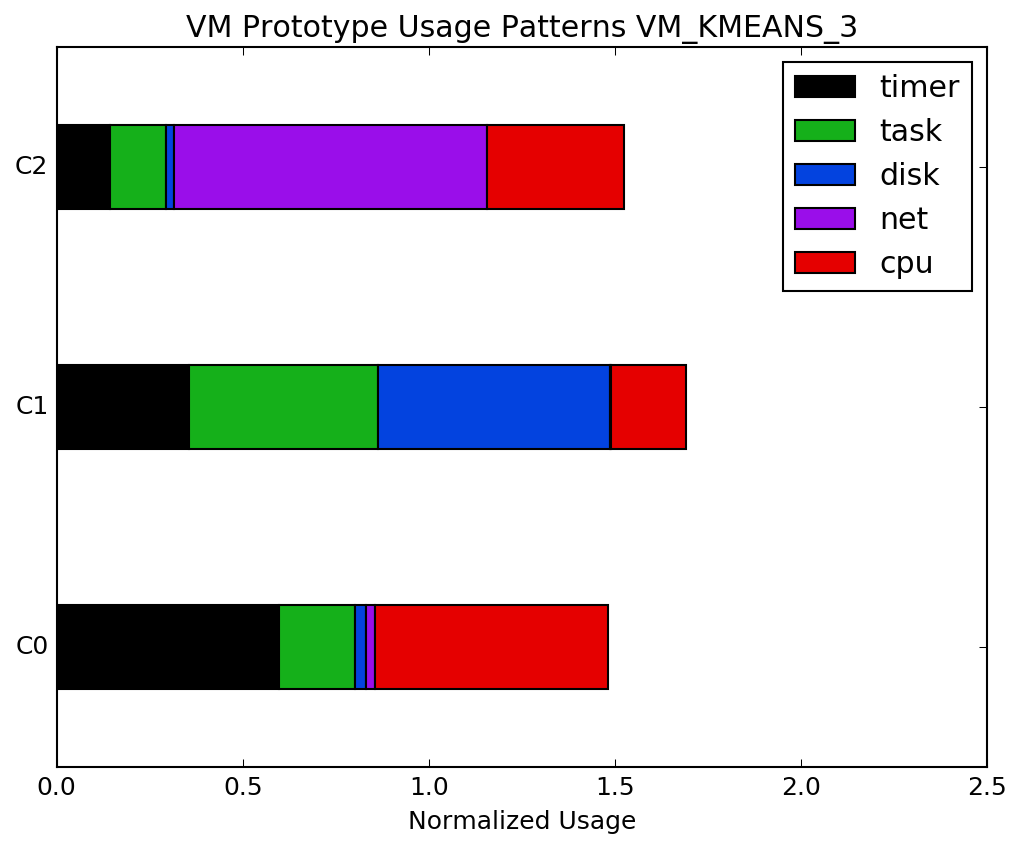
\includegraphics[width=0.45\textwidth]{figs/VM_KMEANS_3_centroids.png}
\caption{Characteristic of Workloads Discovered in First Stage of Clustering}
\label{fig:1st-centroids}
\end{figure}
%%%%%%%%%%%%%%%%%%%%%%%%%%%%
Discuss the centroids found and say what each represents and why these are interesting. Also how we got to this three clusters by taking the one with the best silhouette score. 

%%%%%%%%%%%%%%%%%%%%%%%%%
\begin{figure*}[!htpb]
\centering
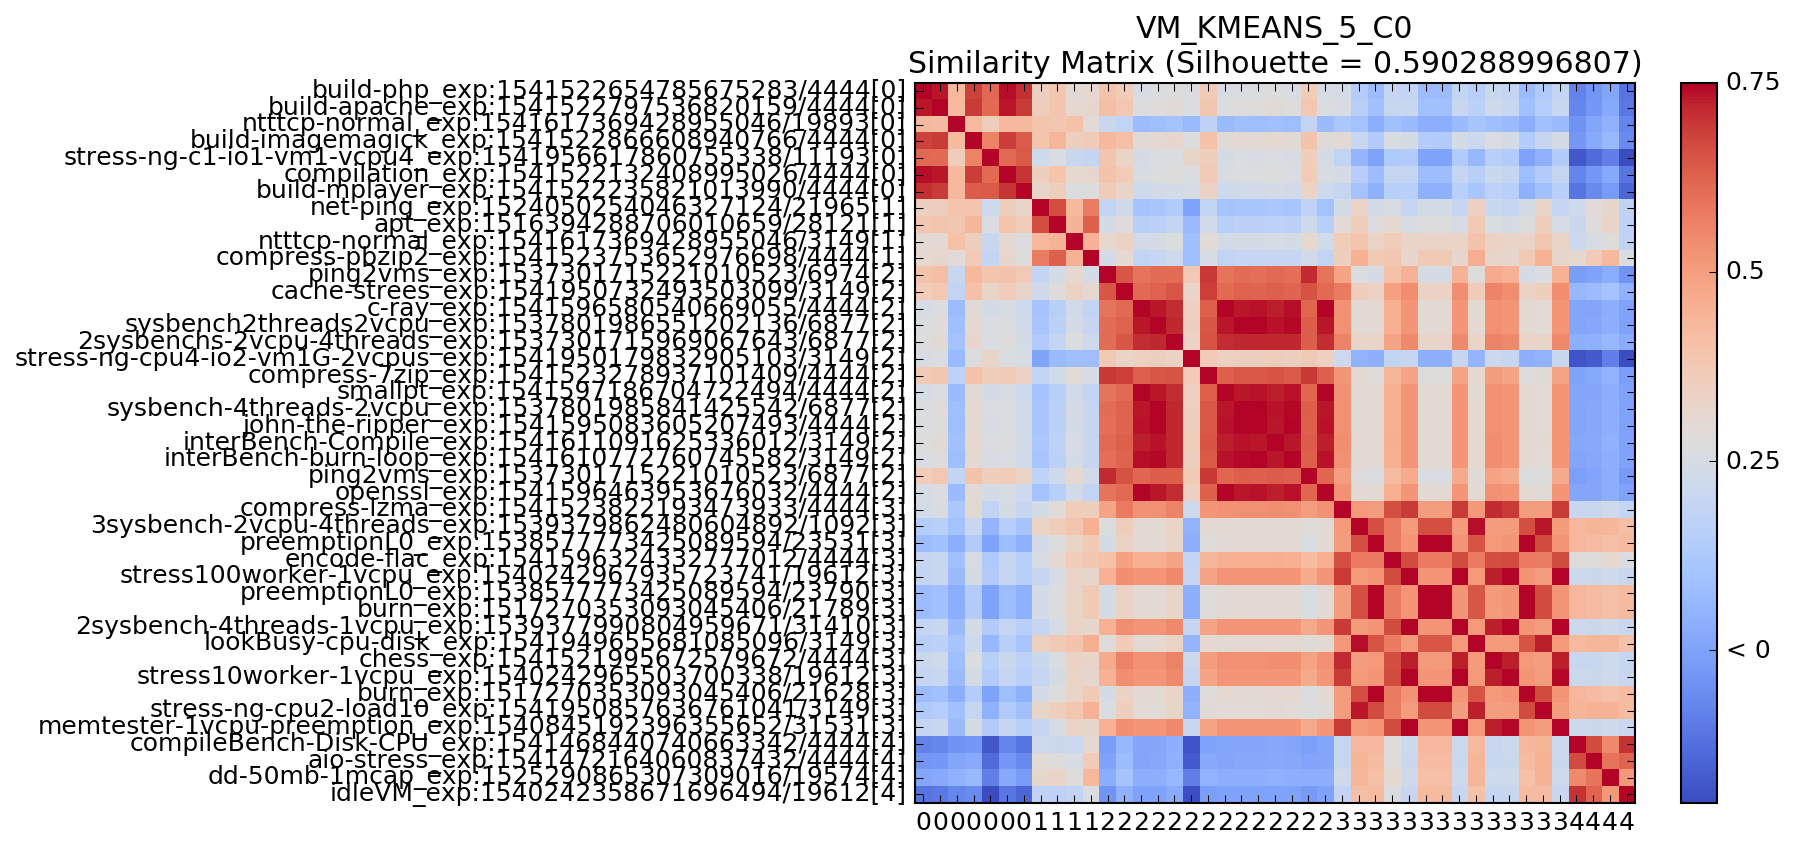
\includegraphics[width=\textwidth]{figs/VM_KMEANS_5_C0.png}
\caption{Similarity Plot For the Five Workload Clusters Discovered in the First Group}
\label{fig:c0-sim}
\end{figure*}
%%%%%%%%%%%%%%%%%%%%%%%%%%%%
Then use similarity plot to say how good or bad the first group is clustered: note how c2 is packed but c3 or c1 is not and explain. Consider overlapping c2 and c3 and explain why that happens and if it reveals some interesting information (Hani?)

%%%%%%%%%%%%%%%%%%%%%%%%%
\begin{figure*}[!htpb]
\centering
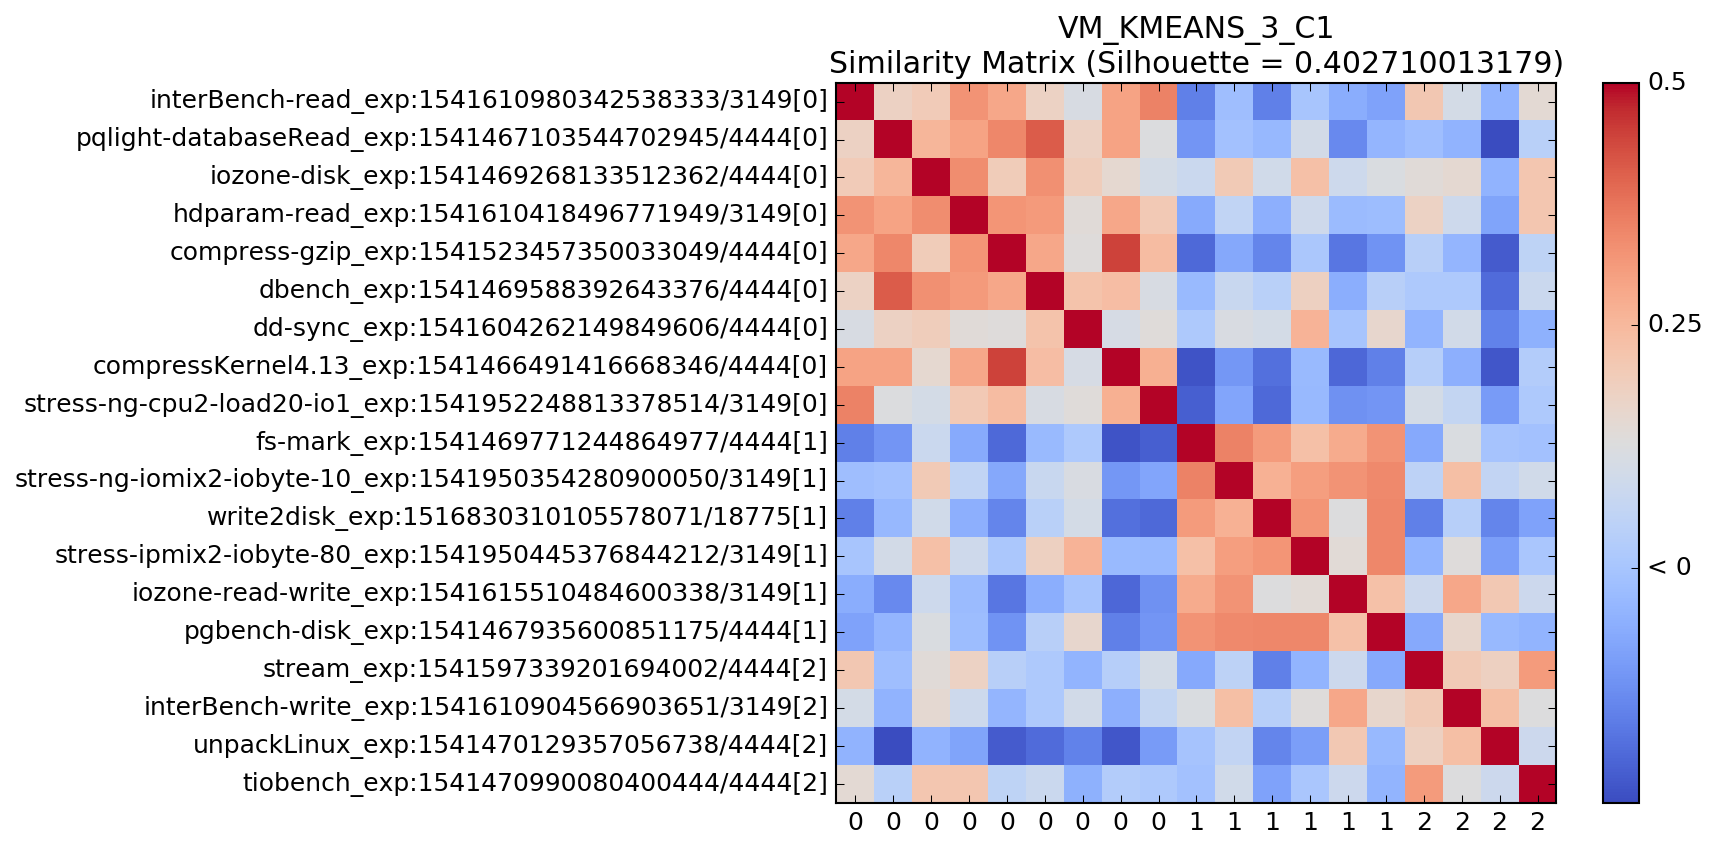
\includegraphics[width=\textwidth]{figs/VM_KMEANS_3_C1.png}
\caption{Similarity Plot For the Three Workload Clusters Discovered in the Second Group}
\label{fig:c1-sim}
\end{figure*}
%%%%%%%%%%%%%%%%%%%%%%%%%%%%
Do the same for second group. More fuzzy group. In particular C2 is very much like noise and uninteresting VM workload. What does this exactly mean for a data center admin? elaborate. 

%%%%%%%%%%%%%%%%%%%%%%%%%
\begin{figure*}[!htpb]
\centering
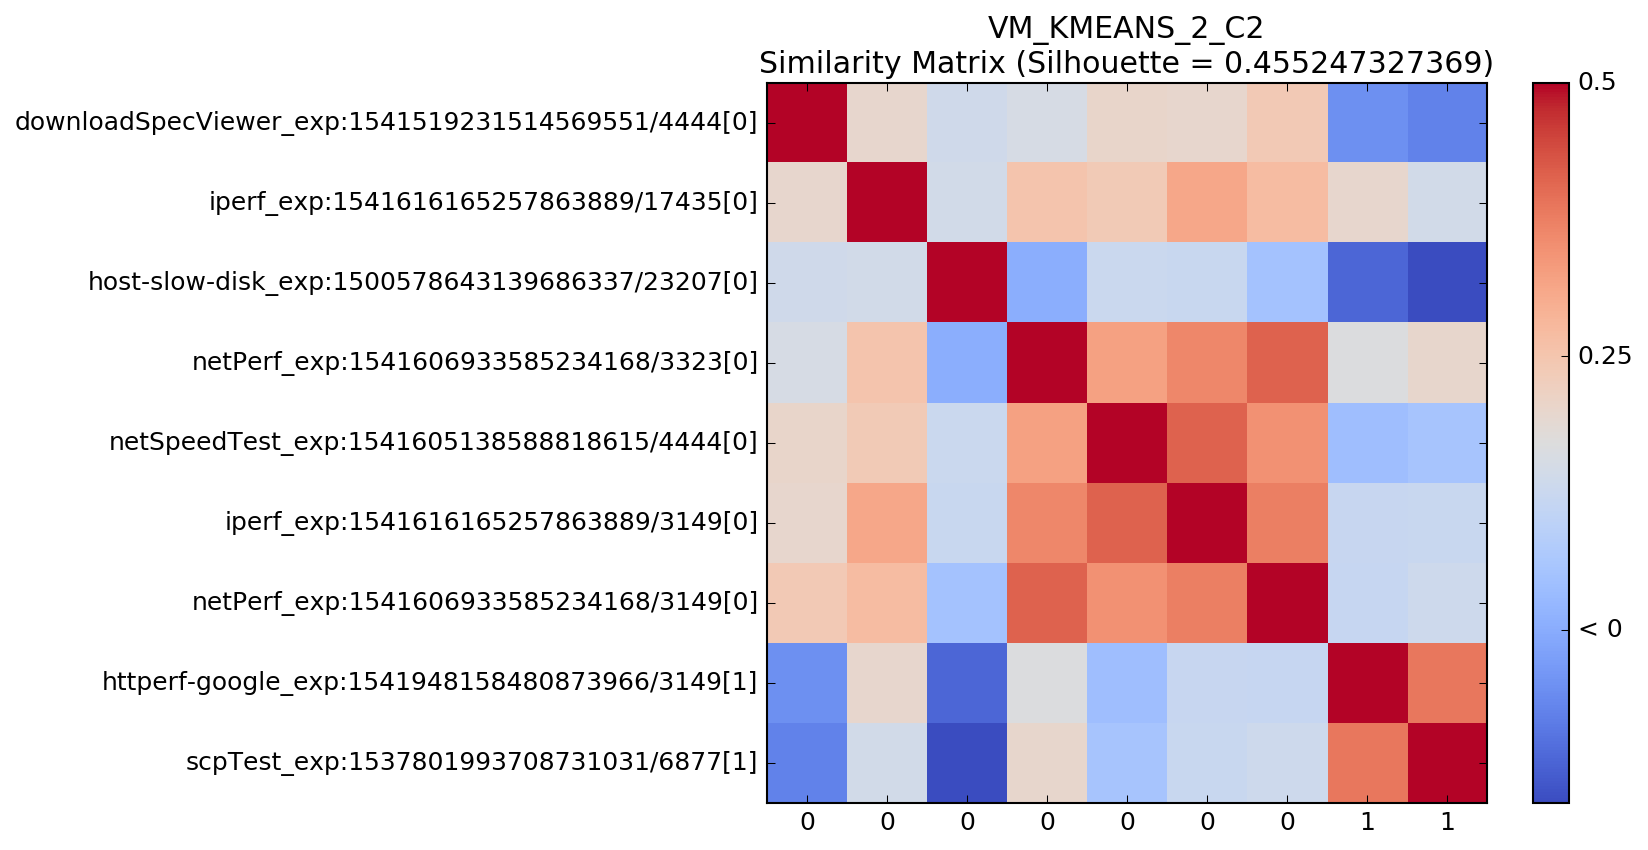
\includegraphics[width=\textwidth]{figs/VM_KMEANS_2_C2.png}
\caption{Similarity Plot For the Two Workload Clusters Discovered in the Third Group}
\label{fig:c2-sim}
\end{figure*}
%%%%%%%%%%%%%%%%%%%%%%%%%%%%
Again the same for third group.

%%%%%%%%%%%%%%%%%%%%%%
\begin{figure*}
	\begin{subfigure}
		\centering
		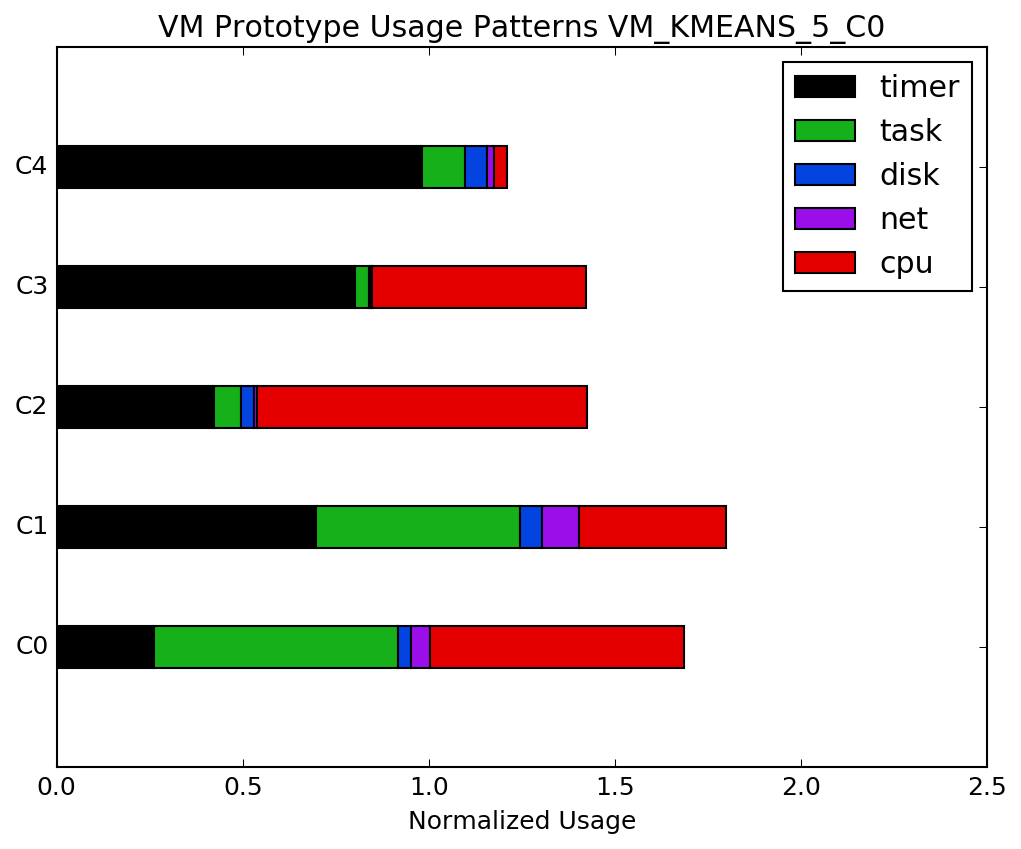
\includegraphics[width=0.3\textwidth]{figs/VM_KMEANS_5_C0_centroids.png}
		\label{fig:c0-centroids}
	\end{subfigure}%
	\begin{subfigure}
		\centering
		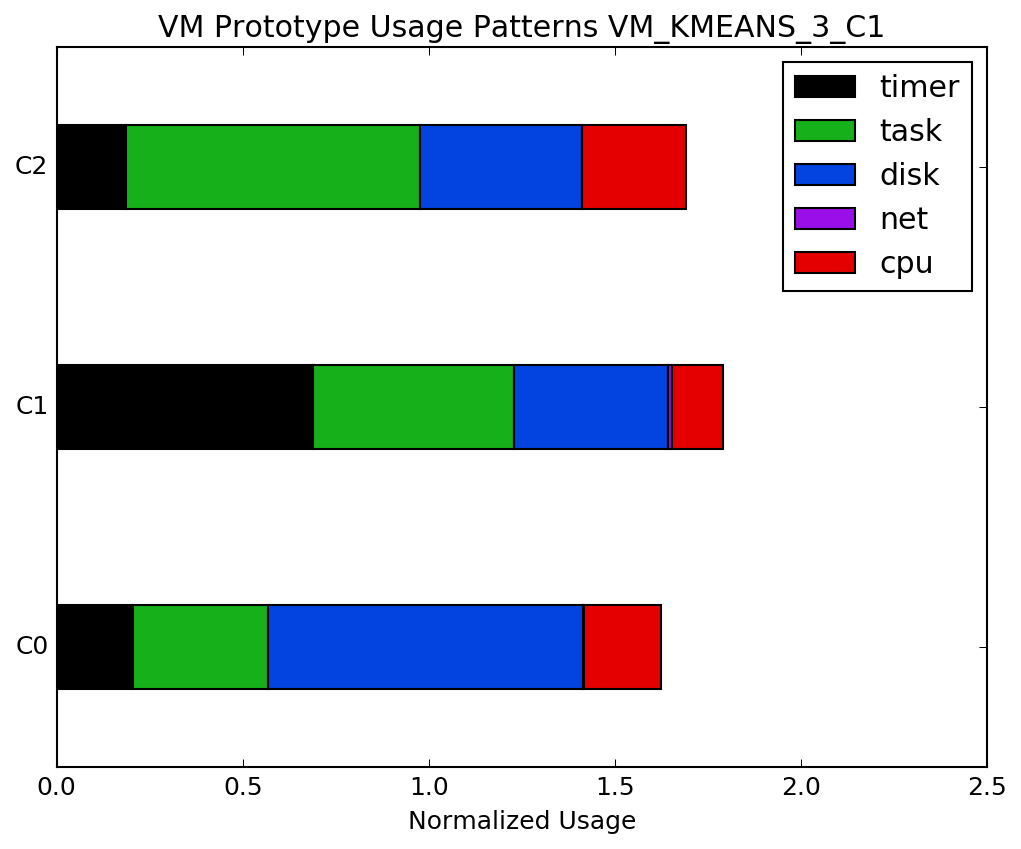
\includegraphics[width=0.3\textwidth]{figs/VM_KMEANS_3_C1_centroids.png}
		\label{fig:c1-centroids}
	\end{subfigure}%
	\begin{subfigure}
		\centering
		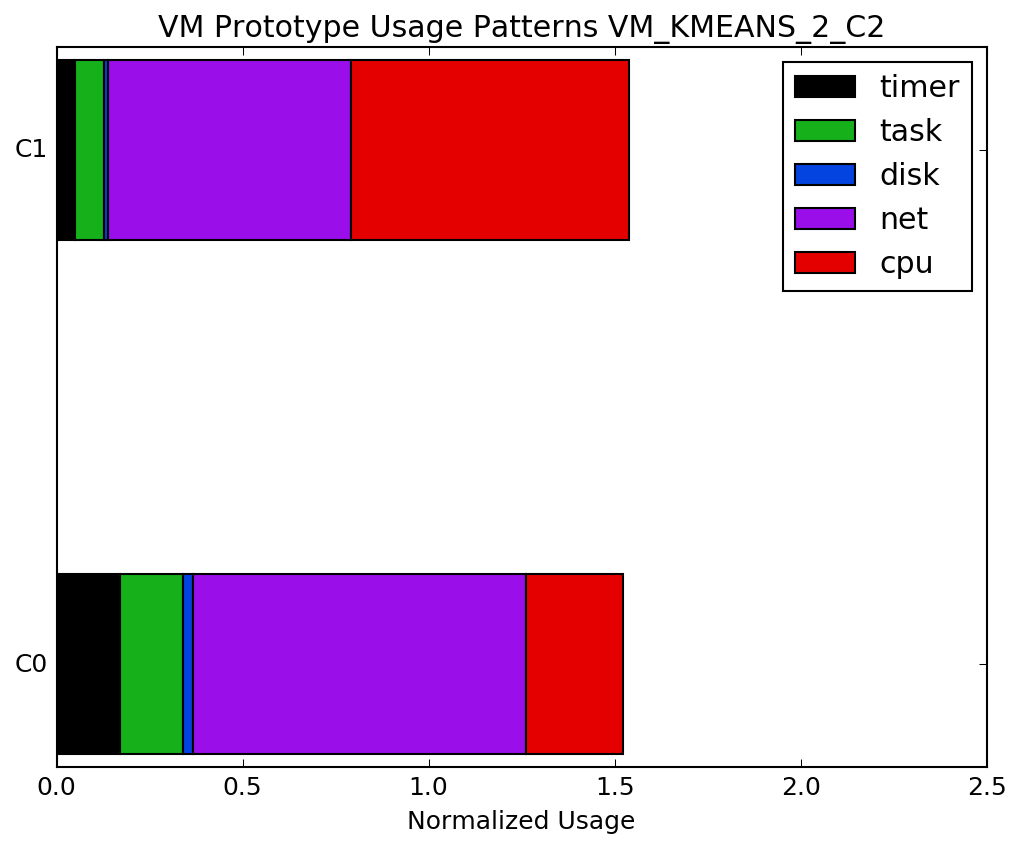
\includegraphics[width=0.3\textwidth]{figs/VM_KMEANS_2_C2_centroids.png}
		\label{fig:c2-centroids}
	\end{subfigure}%
	\caption{Characteristic of Workloads Discovered in Second Stage of Clustering}
	\label{fig:2nd-centroids}
\end{figure*}
%%%%%%%%%%%%%%%%%%%%%%
Now talk about the centroids and how they represent the workload for each cluster.point to interesting and very contrasting cases. How can we take advantage of these diagrams in real life? elaborate (Hani?)

%%%%%%%%%%%%%%%%%%%%%%
\begin{figure*}
	\begin{subfigure}
		\centering
		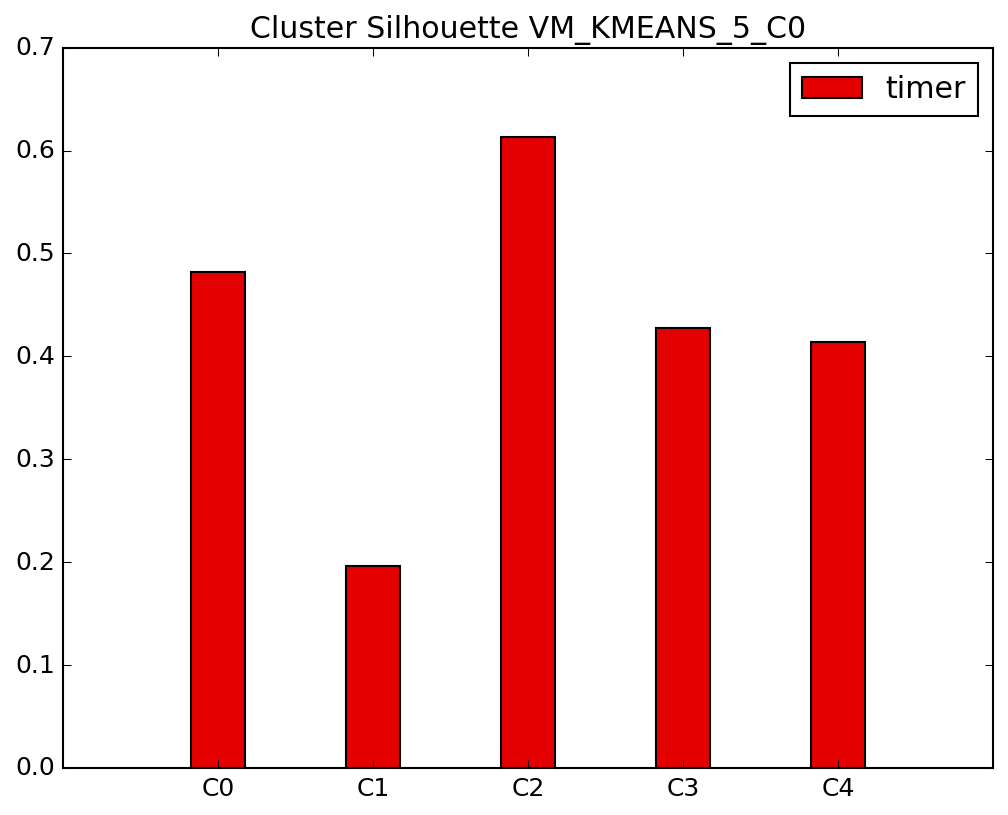
\includegraphics[width=0.3\textwidth]{figs/VM_KMEANS_5_C0_sil.png}
		\label{fig:c0-sil}
	\end{subfigure}%
	\begin{subfigure}
		\centering
		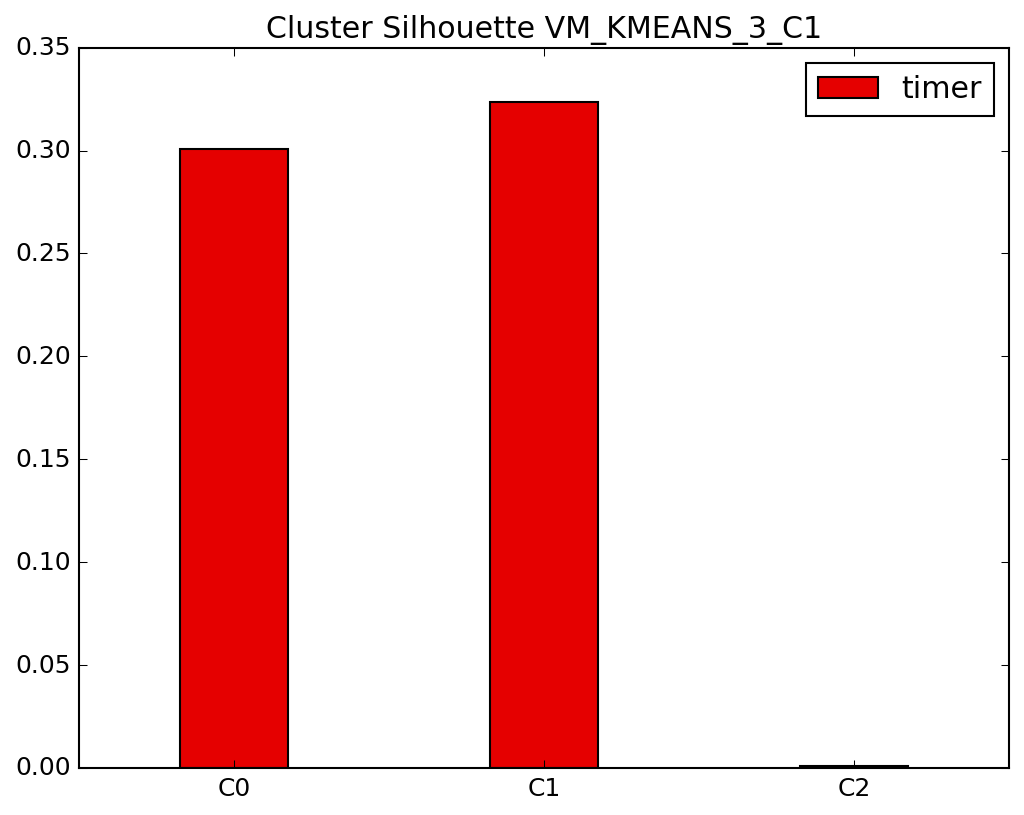
\includegraphics[width=0.3\textwidth]{figs/VM_KMEANS_3_C1_sil.png}
		\label{fig:c1-sil}
	\end{subfigure}%
	\begin{subfigure}
		\centering
		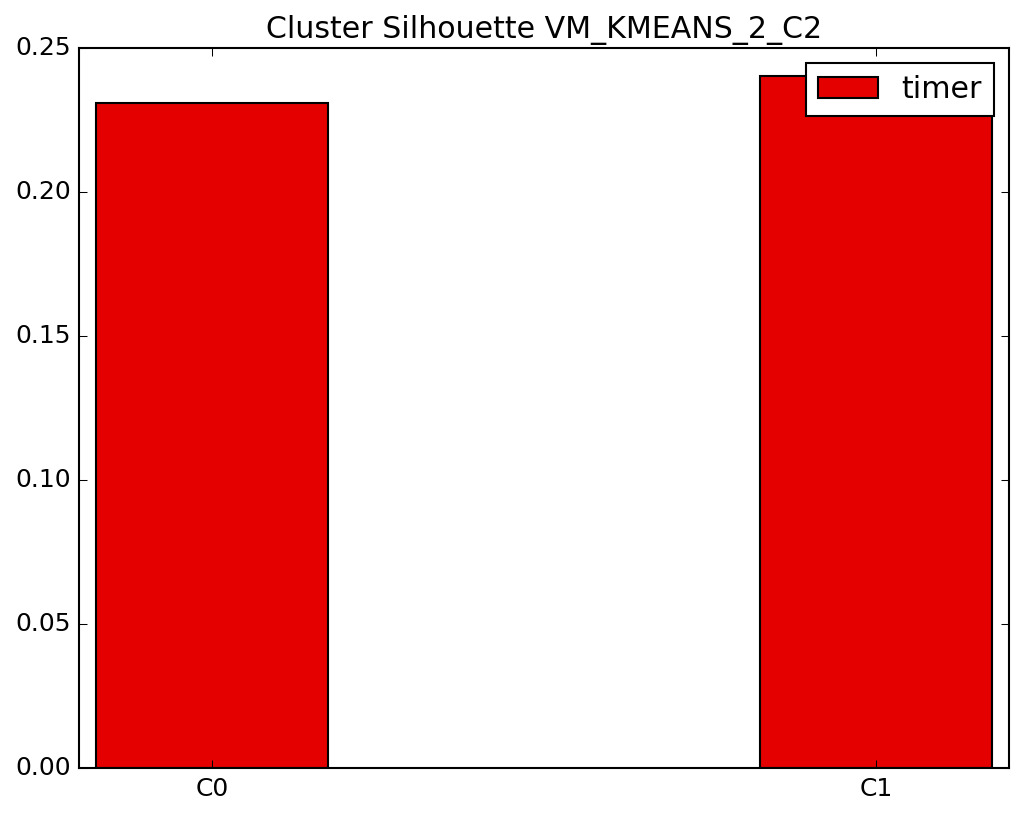
\includegraphics[width=0.3\textwidth]{figs/VM_KMEANS_2_C2_sil.png}
		\label{fig:c2-sil}
	\end{subfigure}%
	\caption{Silhouette Score of VM Clusters Discovered in Second Stage of Clustering}
	\label{fig:2nd-sil}
\end{figure*}
%%%%%%%%%%%%%%%%%%%%%%
These figures \ref{fig:2nd-sil} can assist explaining the similarity matrices. 

%%%%%%%%%%%%%%%%%%%%%%%%%%%%%%%%%%%%%%%%%%%%%%%%%%%%%%%%%%%%%%%%%%%%%%%%%%%%%%%%

\section{Conclusions}






%%%%%%%%%%%%%%%%%%%%%%%%%%%%%%%%%%%%%%%%%%%%%%%%%%%%%%%%%%%%%%%%%%%%%%%%%%%%%%%%
\section*{Acknowledgment}

We would like to gratefully acknowledge the Natural Sciences and Engineering Research Council of Canada (NSERC), Ericsson, Ciena, and EffciOS for funding this project. We thank Genevieve Bastien for her comments.



%%%%%%%%%%%%%%%%%%%%%%%%%%%%%%%%%%%%%%%%%%%%%%%%%%%%%%%%%%%%%%%%%%%%%%%%%%%%%%%%
\bibliographystyle{IEEEtran}
\bibliography{hani}




\end{document}
